\documentclass[10pt]{article}
\usepackage{graphicx}
\usepackage[none]{hyphenat}
\usepackage{listings}
\usepackage[english]{babel}
\usepackage{siunitx}
\usepackage{caption}
\usepackage{booktabs}
\usepackage{array}
\usepackage{extarrows}
\usepackage{enumerate}
\usepackage{enumitem}
\usepackage{amsmath}
\usepackage{commath}
\usepackage{gensymb}
\usepackage{amssymb}
\usepackage{multicol}
\usepackage[utf8]{inputenc}
\lstset{
 frame=single,
 breaklines=true
}
\usepackage{hyperref}
%\usepackage[margin=0.8in]{geometry}
%\usepackage{exsheets}% also loads the `tasks' package
\usepackage{atbegshi}
\AtBeginDocument{\AtBeginShipoutNext{\AtBeginShipoutDiscard}}

%new macro definitions
\renewcommand{\labelenumi}{(\alph{enumi})}
\newcommand{\mydet}[1]{\ensuremath{\begin{vmatrix}#1\end{vmatrix}}}
\providecommand{\brak}[1]{\ensuremath{\left(#1\right)}}
\newcommand{\solution}{\noindent \textbf{Solution: }}
\newcommand{\myvec}[1]{\ensuremath{\begin{pmatrix}#1\end{pmatrix}}}
\providecommand{\norm}[1]{\left\1Vert#1\right\rVert}
\let\vec\mathbf{}


%\SetEnumitemKey{twocol}{
% before=\raggedcolumns\begin{multicols}{2},
% after=\end{multicols}}
%\SetEnumitemKey{fourcol}{
% before=\raggedcolumns\begin{multicols}{4},
% after=\end{multicols}} 


\begin{document}
\begin{center}
\title{\textbf{STRAIGHT LINES}}
\date{\vspace{-5ex}}
\maketitle
\end{center}
\section*{11$^{th}$Math - Chapter 10}
This is Problem-8 from Exercise 10.4\\\\
Find the area of triangle formed by the lines $y-x=0,x+y=0, \text{ and } x-k=0$.

\solution
Given line equations are 
\begin{align}
y-x=0
\label{eq:1}\\
x+y=0
\label{eq:2}\\
x-k=0
\label{eq:3}
\end{align}
\begin{figure}[!h]
	\begin{center}
		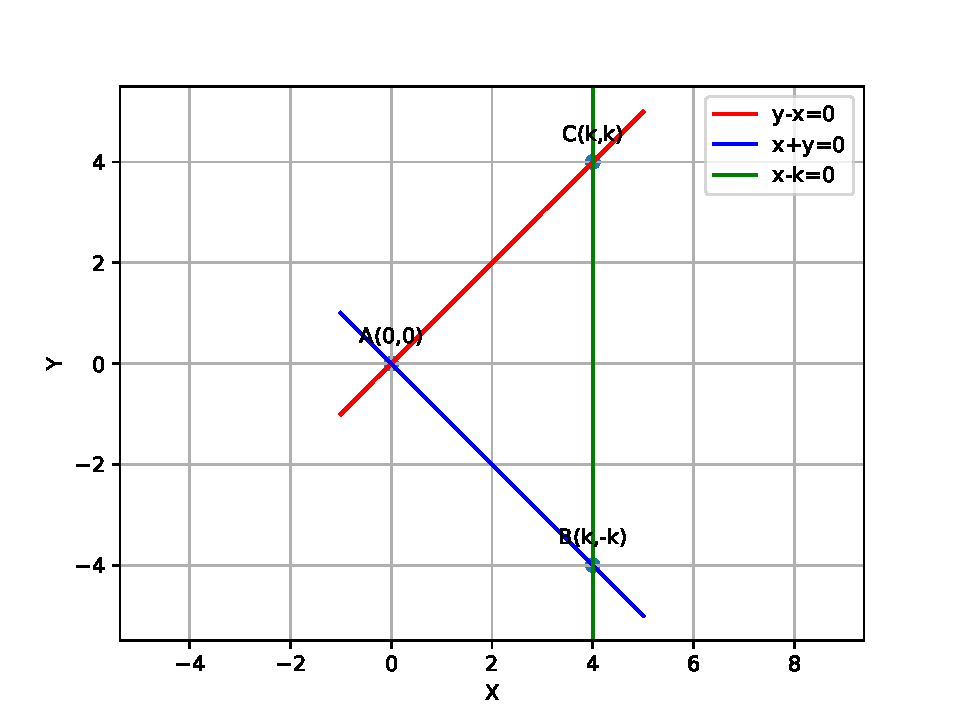
\includegraphics[width=\columnwidth]{./figs/fig.pdf}
	\end{center}
\caption{}
\label{figure}
\end{figure}
These \eqref{eq:1},\eqref{eq:2},\eqref{eq:3} line equations intersect at points A,B,C.\\
from graph,\\
\begin{align}
	A&=\myvec{0\\0}\\
	B&=\myvec{k\\-k} \\
	C&=\myvec{k\\k}
\end{align}
We know that
\begin{align}
ar(ABC) &=\frac{1}{2}\norm{(A-B)\times(A-C)}\\
	&=\frac{1}{2}\norm{\brak{\myvec{0\\0}-\myvec{k\\-k}}\times\brak{\myvec{0\\0}-\myvec{k\\k}}}\\
	&=\frac{1}{2}\norm{\myvec{-k\\k}\times\myvec{-k\\-k}}\\
	&=\frac{1}{2}\norm{2k^2}\\
\implies &=k^2
\end{align}
\end{document}
